\PassOptionsToPackage{unicode=true}{hyperref} % options for packages loaded elsewhere
\PassOptionsToPackage{hyphens}{url}
%
\documentclass[ignorenonframetext,]{beamer}
\usepackage{pgfpages}
\setbeamertemplate{caption}[numbered]
\setbeamertemplate{caption label separator}{: }
\setbeamercolor{caption name}{fg=normal text.fg}
\beamertemplatenavigationsymbolsempty
\usepackage{lmodern}
\usepackage{amssymb,amsmath}
\usepackage{ifxetex,ifluatex}
\usepackage{fixltx2e} % provides \textsubscript
\ifnum 0\ifxetex 1\fi\ifluatex 1\fi=0 % if pdftex
  \usepackage[T1]{fontenc}
  \usepackage[utf8]{inputenc}
  \usepackage{textcomp} % provides euro and other symbols
\else % if luatex or xelatex
  \usepackage{unicode-math}
  \defaultfontfeatures{Ligatures=TeX,Scale=MatchLowercase}
\fi
\usetheme[]{CambridgeUS}
\usecolortheme{beaver}
\usefonttheme{structurebold}
% use upquote if available, for straight quotes in verbatim environments
\IfFileExists{upquote.sty}{\usepackage{upquote}}{}
% use microtype if available
\IfFileExists{microtype.sty}{%
\usepackage[]{microtype}
\UseMicrotypeSet[protrusion]{basicmath} % disable protrusion for tt fonts
}{}
\IfFileExists{parskip.sty}{%
\usepackage{parskip}
}{% else
\setlength{\parindent}{0pt}
\setlength{\parskip}{6pt plus 2pt minus 1pt}
}
\usepackage{hyperref}
\hypersetup{
            pdftitle={B2 Das osmdata Paket},
            pdfauthor={Jan-Philipp Kolb},
            pdfborder={0 0 0},
            breaklinks=true}
\urlstyle{same}  % don't use monospace font for urls
\newif\ifbibliography
\usepackage{color}
\usepackage{fancyvrb}
\newcommand{\VerbBar}{|}
\newcommand{\VERB}{\Verb[commandchars=\\\{\}]}
\DefineVerbatimEnvironment{Highlighting}{Verbatim}{commandchars=\\\{\}}
% Add ',fontsize=\small' for more characters per line
\usepackage{framed}
\definecolor{shadecolor}{RGB}{248,248,248}
\newenvironment{Shaded}{\begin{snugshade}}{\end{snugshade}}
\newcommand{\AlertTok}[1]{\textcolor[rgb]{0.94,0.16,0.16}{#1}}
\newcommand{\AnnotationTok}[1]{\textcolor[rgb]{0.56,0.35,0.01}{\textbf{\textit{#1}}}}
\newcommand{\AttributeTok}[1]{\textcolor[rgb]{0.77,0.63,0.00}{#1}}
\newcommand{\BaseNTok}[1]{\textcolor[rgb]{0.00,0.00,0.81}{#1}}
\newcommand{\BuiltInTok}[1]{#1}
\newcommand{\CharTok}[1]{\textcolor[rgb]{0.31,0.60,0.02}{#1}}
\newcommand{\CommentTok}[1]{\textcolor[rgb]{0.56,0.35,0.01}{\textit{#1}}}
\newcommand{\CommentVarTok}[1]{\textcolor[rgb]{0.56,0.35,0.01}{\textbf{\textit{#1}}}}
\newcommand{\ConstantTok}[1]{\textcolor[rgb]{0.00,0.00,0.00}{#1}}
\newcommand{\ControlFlowTok}[1]{\textcolor[rgb]{0.13,0.29,0.53}{\textbf{#1}}}
\newcommand{\DataTypeTok}[1]{\textcolor[rgb]{0.13,0.29,0.53}{#1}}
\newcommand{\DecValTok}[1]{\textcolor[rgb]{0.00,0.00,0.81}{#1}}
\newcommand{\DocumentationTok}[1]{\textcolor[rgb]{0.56,0.35,0.01}{\textbf{\textit{#1}}}}
\newcommand{\ErrorTok}[1]{\textcolor[rgb]{0.64,0.00,0.00}{\textbf{#1}}}
\newcommand{\ExtensionTok}[1]{#1}
\newcommand{\FloatTok}[1]{\textcolor[rgb]{0.00,0.00,0.81}{#1}}
\newcommand{\FunctionTok}[1]{\textcolor[rgb]{0.00,0.00,0.00}{#1}}
\newcommand{\ImportTok}[1]{#1}
\newcommand{\InformationTok}[1]{\textcolor[rgb]{0.56,0.35,0.01}{\textbf{\textit{#1}}}}
\newcommand{\KeywordTok}[1]{\textcolor[rgb]{0.13,0.29,0.53}{\textbf{#1}}}
\newcommand{\NormalTok}[1]{#1}
\newcommand{\OperatorTok}[1]{\textcolor[rgb]{0.81,0.36,0.00}{\textbf{#1}}}
\newcommand{\OtherTok}[1]{\textcolor[rgb]{0.56,0.35,0.01}{#1}}
\newcommand{\PreprocessorTok}[1]{\textcolor[rgb]{0.56,0.35,0.01}{\textit{#1}}}
\newcommand{\RegionMarkerTok}[1]{#1}
\newcommand{\SpecialCharTok}[1]{\textcolor[rgb]{0.00,0.00,0.00}{#1}}
\newcommand{\SpecialStringTok}[1]{\textcolor[rgb]{0.31,0.60,0.02}{#1}}
\newcommand{\StringTok}[1]{\textcolor[rgb]{0.31,0.60,0.02}{#1}}
\newcommand{\VariableTok}[1]{\textcolor[rgb]{0.00,0.00,0.00}{#1}}
\newcommand{\VerbatimStringTok}[1]{\textcolor[rgb]{0.31,0.60,0.02}{#1}}
\newcommand{\WarningTok}[1]{\textcolor[rgb]{0.56,0.35,0.01}{\textbf{\textit{#1}}}}
\usepackage{graphicx,grffile}
\makeatletter
\def\maxwidth{\ifdim\Gin@nat@width>\linewidth\linewidth\else\Gin@nat@width\fi}
\def\maxheight{\ifdim\Gin@nat@height>\textheight\textheight\else\Gin@nat@height\fi}
\makeatother
% Scale images if necessary, so that they will not overflow the page
% margins by default, and it is still possible to overwrite the defaults
% using explicit options in \includegraphics[width, height, ...]{}
\setkeys{Gin}{width=\maxwidth,height=\maxheight,keepaspectratio}
% Prevent slide breaks in the middle of a paragraph:
\widowpenalties 1 10000
\raggedbottom
\setbeamertemplate{part page}{
\centering
\begin{beamercolorbox}[sep=16pt,center]{part title}
  \usebeamerfont{part title}\insertpart\par
\end{beamercolorbox}
}
\setbeamertemplate{section page}{
\centering
\begin{beamercolorbox}[sep=12pt,center]{part title}
  \usebeamerfont{section title}\insertsection\par
\end{beamercolorbox}
}
\setbeamertemplate{subsection page}{
\centering
\begin{beamercolorbox}[sep=8pt,center]{part title}
  \usebeamerfont{subsection title}\insertsubsection\par
\end{beamercolorbox}
}
\AtBeginPart{
  \frame{\partpage}
}
\AtBeginSection{
  \ifbibliography
  \else
    \frame{\sectionpage}
  \fi
}
\AtBeginSubsection{
  \frame{\subsectionpage}
}
\setlength{\emergencystretch}{3em}  % prevent overfull lines
\providecommand{\tightlist}{%
  \setlength{\itemsep}{0pt}\setlength{\parskip}{0pt}}
\setcounter{secnumdepth}{0}

<<<<<<< HEAD
\title{B2 Das \texttt{osmdata} Paket}
=======
% set default figure placement to htbp
\makeatletter
\def\fps@figure{htbp}
\makeatother


\title{Das \texttt{osmdata} Paket}
>>>>>>> 7c70862562048dd83d35abf8915c3b64447f18d2
\author{Jan-Philipp Kolb}
\date{22 Oktober 2018}

\begin{document}
\frame{\titlepage}

\begin{frame}[fragile]{Themen dieses Abschnitts}
\protect\hypertarget{themen-dieses-abschnitts}{}

\begin{itemize}
\tightlist
\item
  Die
  \href{https://wiki.openstreetmap.org/wiki/Overpass_API}{\textbf{Overpass
  API}} von Roland Olbricht wird vorgestellt.
\end{itemize}

\begin{itemize}
\item
  Das R-Paket \texttt{osmdata} mit dem man OSM-Daten herunterladen kann
  und das auf der
  \href{https://wiki.openstreetmap.org/wiki/Overpass_API}{\textbf{Overpass
  API}} beruht.
\item
  Die Verarbeitung der OSM-Daten mit dem Paket simple features
  (\texttt{sf})
\item
  Wie man die OSM Daten graphisch darstellen kann.
\end{itemize}

\end{frame}

\begin{frame}{\href{https://overpass-turbo.eu/}{Overpass Turbo}}
\protect\hypertarget{overpass-turbo}{}

\begin{figure}
\centering
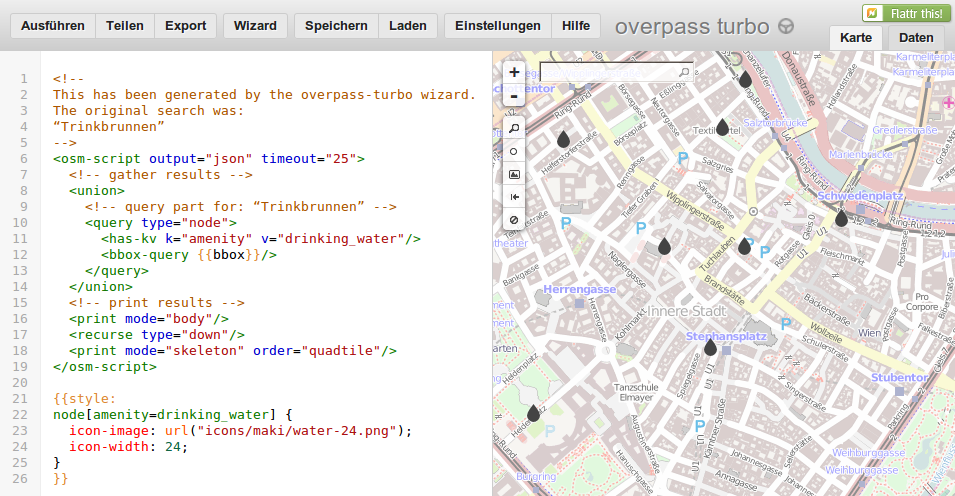
\includegraphics{figure/Overpass_turbo_query_wizard_result_DE.png}
\caption{\url{https://overpass-turbo.eu/}}
\end{figure}

\end{frame}

\begin{frame}[fragile]{Query Overpass}
\protect\hypertarget{query-overpass}{}

\begin{itemize}
\tightlist
\item
  In der folgenden Abfrage wird bei Overpass Turbo nach Bars im
  ausgewählten Fenster gesucht.
\end{itemize}

\begin{verbatim}
node
  [amenity=bar]
  ({{bbox}});
out;
\end{verbatim}

\end{frame}

\begin{frame}{Export bei Overpass}
\protect\hypertarget{export-bei-overpass}{}

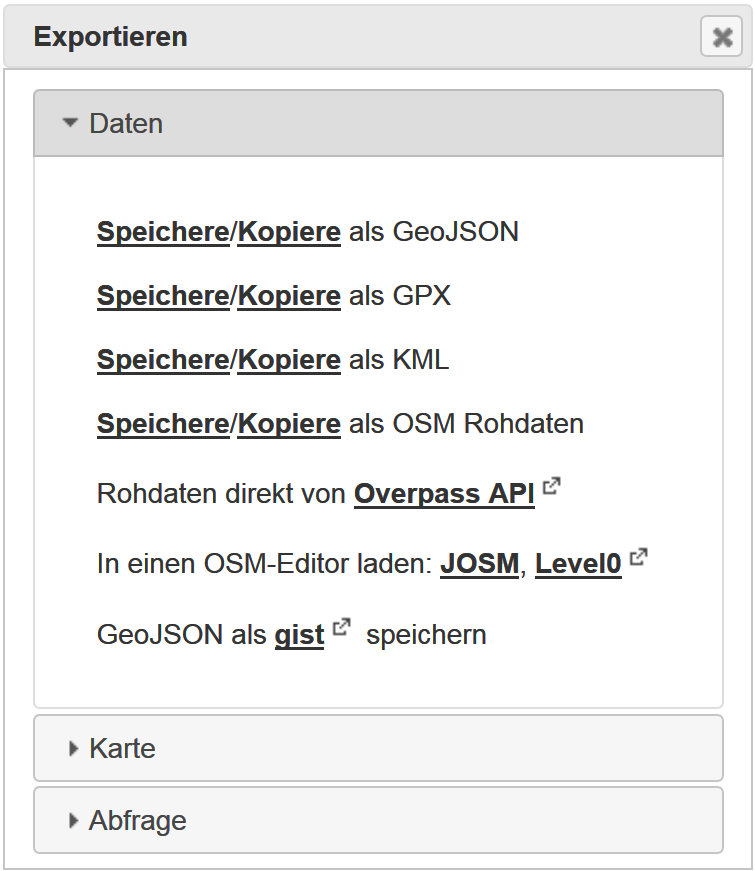
\includegraphics{figure/OverpassExport.PNG}

\end{frame}

\begin{frame}{Speicherformate}
\protect\hypertarget{speicherformate}{}

\begin{block}{Bei Export von Overpass}

\begin{itemize}
\tightlist
\item
  GeoJSON
\item
  GPX
\item
  KML
\item
  OSM Rohdaten
\end{itemize}

\end{block}

\end{frame}

\begin{frame}{Import von Daten}
\protect\hypertarget{import-von-daten}{}

\end{frame}

\begin{frame}{\href{https://github.com/ropensci/osmdata}{Das
\texttt{osmdata} Paket}}
\protect\hypertarget{das-osmdata-paket}{}


\includegraphics{figure/osmdatatitle.png}

\begin{quote}
Mark Padgham - Import `OpenStreetMap' Data as Simple Features or Spatial
Objects
\end{quote}

\end{frame}

\begin{frame}[fragile]{Das \texttt{osmdata} Paket}
\protect\hypertarget{das-osmdata-paket-1}{}

\begin{itemize}
\tightlist
\item
  Mit dem Paket kann man Daten von OpenStreetMap importieren
\item
  Die OSM Daten sind unter
  \href{https://www.openstreetmap.org/copyright}{\textbf{ODbL licence}}
  zu haben
\end{itemize}

\begin{Shaded}
\begin{Highlighting}[]
\KeywordTok{install.packages}\NormalTok{(}\StringTok{"osmdata"}\NormalTok{)}
\end{Highlighting}
\end{Shaded}

\begin{Shaded}
\begin{Highlighting}[]
\KeywordTok{library}\NormalTok{(osmdata)}
\end{Highlighting}
\end{Shaded}

\begin{Shaded}
\begin{Highlighting}[]
\KeywordTok{citation}\NormalTok{(}\StringTok{"osmdata"}\NormalTok{)}
\end{Highlighting}
\end{Shaded}

\end{frame}

\begin{frame}[fragile]{Das Paket \texttt{osmplotr}}
\protect\hypertarget{das-paket-osmplotr}{}

\begin{Shaded}
\begin{Highlighting}[]
\KeywordTok{library}\NormalTok{(}\StringTok{"osmplotr"}\NormalTok{)}
\KeywordTok{library}\NormalTok{(}\StringTok{"osmdata"}\NormalTok{)}
\end{Highlighting}
\end{Shaded}

\end{frame}

\begin{frame}[fragile]{Beispiel Kindergärten in Mannheim}
\protect\hypertarget{beispiel-kindergarten-in-mannheim}{}

\begin{Shaded}
\begin{Highlighting}[]
\NormalTok{bbox <-}\StringTok{ }\KeywordTok{getbb}\NormalTok{(}\StringTok{"Mannheim"}\NormalTok{)}
\NormalTok{dat_osm <-}\StringTok{ }\KeywordTok{extract_osm_objects}\NormalTok{(}\DataTypeTok{key=}\StringTok{'building'}\NormalTok{, }
                              \DataTypeTok{value=}\StringTok{"kindergarten"}\NormalTok{,}
                              \DataTypeTok{bbox=}\NormalTok{bbox)}
\end{Highlighting}
\end{Shaded}

\end{frame}

\begin{frame}[fragile]{Einen Rahmen definieren um Daten zu bekommen}
\protect\hypertarget{einen-rahmen-definieren-um-daten-zu-bekommen}{}

\begin{itemize}
\tightlist
\item
  Der Rahmen kann entweder erstellt werden, indem die Koordinaten
  angegeben werden:
\end{itemize}

\begin{Shaded}
\begin{Highlighting}[]
\NormalTok{q <-}\StringTok{ }\KeywordTok{opq}\NormalTok{(}\DataTypeTok{bbox =} \KeywordTok{c}\NormalTok{(}\FloatTok{52.3}\NormalTok{, }\FloatTok{4.7}\NormalTok{, }\FloatTok{52.4}\NormalTok{, }\FloatTok{5.1}\NormalTok{))}
\end{Highlighting}
\end{Shaded}

\begin{itemize}
\tightlist
\item
  oder indem man den Befehl \texttt{getbb} verwendet:
\end{itemize}

\begin{Shaded}
\begin{Highlighting}[]
\NormalTok{bb <-}\StringTok{ }\KeywordTok{getbb}\NormalTok{(}\StringTok{'Ladenburg'}\NormalTok{)}
\end{Highlighting}
\end{Shaded}

\begin{itemize}
\item
  In \texttt{bb} sind nun vier Werte gespeichert, die den Rahmen
  definieren
\item
  Befehl \texttt{opq} - eine Overpass Anfrage erstellen
\end{itemize}

\begin{Shaded}
\begin{Highlighting}[]
\NormalTok{q <-}\StringTok{ }\KeywordTok{opq}\NormalTok{(}\DataTypeTok{bbox =}\NormalTok{ bb)}
\end{Highlighting}
\end{Shaded}

\end{frame}

\begin{frame}[fragile]{Die Grenze von Mannheim}
\protect\hypertarget{die-grenze-von-mannheim}{}

\begin{itemize}
\tightlist
\item
  Erst mit dem Argument \texttt{format\_out=polygon} Befehl
  \texttt{getbb} erhält man das Polygon:
\end{itemize}

\begin{Shaded}
\begin{Highlighting}[]
\NormalTok{bb_poly <-}\StringTok{ }\KeywordTok{getbb}\NormalTok{(}\DataTypeTok{place_name =} \StringTok{"Ladenburg"}\NormalTok{, }
                 \DataTypeTok{format_out =} \StringTok{"polygon"}\NormalTok{)}
\end{Highlighting}
\end{Shaded}

\begin{itemize}
\tightlist
\item
  Das Ergebnis ist sind zwei Vektoren mit den Longitude und Latitude
  Koordinaten.
\end{itemize}

\begin{verbatim}
##          [,1]     [,2]
## [1,] 8.569720 49.49107
## [2,] 8.569858 49.49101
## [3,] 8.569999 49.49096
## [4,] 8.570342 49.49085
\end{verbatim}

\end{frame}

\begin{frame}[fragile]{Das Paket für simple feature (\texttt{sf})}
\protect\hypertarget{das-paket-fur-simple-feature-sf}{}

\begin{quote}
Simple Features for R
\end{quote}

\begin{itemize}
\tightlist
\item
  Das Paket \texttt{sf} ist ein Paket um geometrische Operationen
  durchzuführen.
\end{itemize}

\begin{Shaded}
\begin{Highlighting}[]
\KeywordTok{library}\NormalTok{(sf)}
\end{Highlighting}
\end{Shaded}

\begin{itemize}
\tightlist
\item
  \href{https://cran.r-project.org/web/packages/sf/vignettes/sf3.html}{\textbf{Vignette
  für das Paket \texttt{sf}}}
\end{itemize}

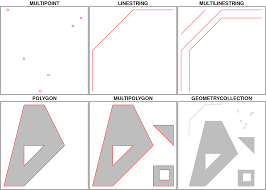
\includegraphics{figure/rsimplefeatures.png}

\end{frame}

\begin{frame}[fragile]{Die Funktion \texttt{st\_linestring}}
\protect\hypertarget{die-funktion-st_linestring}{}

\begin{quote}
Create simple feature from a numeric vector, matrix or list
\end{quote}

\begin{Shaded}
\begin{Highlighting}[]
\KeywordTok{library}\NormalTok{(sf)}
\NormalTok{ls <-}\StringTok{ }\KeywordTok{st_linestring}\NormalTok{(bb_poly)}
\NormalTok{sfc <-}\StringTok{ }\KeywordTok{st_sfc}\NormalTok{(ls)}
\end{Highlighting}
\end{Shaded}

\end{frame}

\begin{frame}[fragile]{Den \texttt{linestring} plotten}
\protect\hypertarget{den-linestring-plotten}{}

\begin{Shaded}
\begin{Highlighting}[]
\KeywordTok{library}\NormalTok{(tmap)}
\KeywordTok{qtm}\NormalTok{(sfc)}
\end{Highlighting}
\end{Shaded}

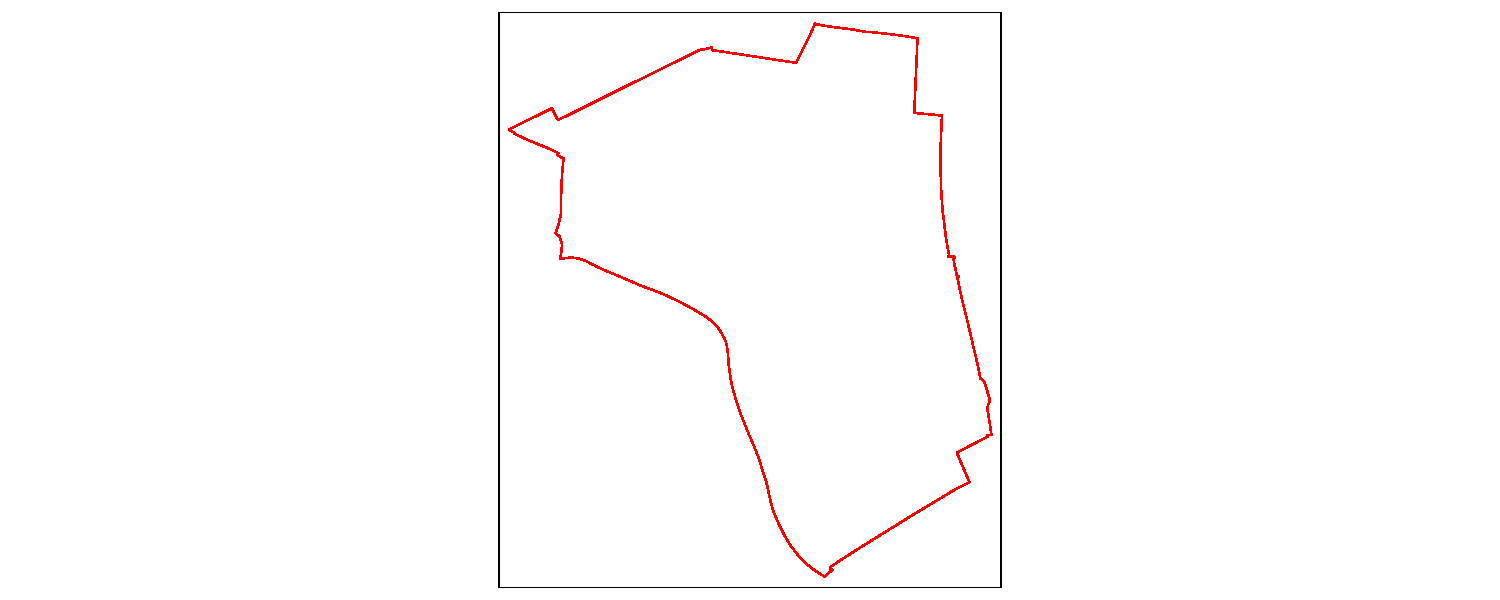
\includegraphics{osmdata_files/figure-beamer/unnamed-chunk-17-1.pdf}

\end{frame}

\begin{frame}[fragile]{Einrichtungen (amenity)}
\protect\hypertarget{einrichtungen-amenity}{}

\begin{block}{\href{https://wiki.openstreetmap.org/wiki/Map_Features}{\textbf{OSM
map features}}}

\begin{itemize}
\item
  Alle benannten Objekte findet man, wenn man OSM map features in eine
  Suchmaschine eingibt.
\item
  Achtung, wenn man bspw. alle Objekte mit dem Schlüssel
  \texttt{amenity} für eine Stadt heraussucht, bekommt man einen recht
  großen Datensatz
\end{itemize}

\begin{Shaded}
\begin{Highlighting}[]
\NormalTok{q <-}\StringTok{ }\KeywordTok{add_osm_feature}\NormalTok{ (q, }\DataTypeTok{key =} \StringTok{'amenity'}\NormalTok{)}
\KeywordTok{osmdata_xml}\NormalTok{(q, }\StringTok{'../data/Ladenburg_amenity.osm'}\NormalTok{)}
\end{Highlighting}
\end{Shaded}

\end{block}

\end{frame}

\begin{frame}{Was dahinter steckt}
\protect\hypertarget{was-dahinter-steckt}{}

\end{frame}

\begin{frame}[fragile]{Die Funktion \texttt{osmdata\_sf}}
\protect\hypertarget{die-funktion-osmdata_sf}{}

\begin{itemize}
\tightlist
\item
  Die Funktion \texttt{osmdata\_sf} gibt ein \texttt{osmdata} ObjeKt im
  \texttt{sf} Format.
\end{itemize}

\begin{Shaded}
\begin{Highlighting}[]
\KeywordTok{library}\NormalTok{(magrittr)}
\NormalTok{dat1 <-}\StringTok{ }\KeywordTok{opq}\NormalTok{(}\DataTypeTok{bbox =} \StringTok{'Ladenburg'}\NormalTok{) }\OperatorTok
\StringTok{    }\KeywordTok{add_osm_feature}\NormalTok{(}\DataTypeTok{key =} \StringTok{'shop'}\NormalTok{, }\DataTypeTok{value =} \StringTok{'bakery'}\NormalTok{) }\OperatorTok
\StringTok{    }\KeywordTok{osmdata_sf}\NormalTok{ ()}
\end{Highlighting}
\end{Shaded}

\begin{Shaded}
\begin{Highlighting}[]
\KeywordTok{unlist}\NormalTok{(}\KeywordTok{lapply}\NormalTok{(dat1,nrow))}
\end{Highlighting}
\end{Shaded}

\begin{verbatim}
##        osm_points         osm_lines      osm_polygons    osm_multilines 
##                16                 0                 0                 0 
## osm_multipolygons 
##                 0
\end{verbatim}

\end{frame}

\begin{frame}[fragile]{Alles in eine Karte plotten}
\protect\hypertarget{alles-in-eine-karte-plotten}{}

\begin{block}{\href{https://cran.r-project.org/web/packages/tmap/vignettes/tmap-getstarted.html}{**Der
Start mit dem Paket \texttt{tmap}}}

\begin{Shaded}
\begin{Highlighting}[]
\KeywordTok{library}\NormalTok{(tmap)}
\KeywordTok{tm_shape}\NormalTok{(sfc) }
\KeywordTok{tm_bubbles}\NormalTok{(dat, }\DataTypeTok{size=}\DecValTok{2}\NormalTok{)}
\end{Highlighting}
\end{Shaded}

\end{block}

\end{frame}

\begin{frame}[fragile]{Beispiel Fahrradparkplätze}
\protect\hypertarget{beispiel-fahrradparkplatze}{}

\begin{itemize}
\tightlist
\item
  \href{https://wiki.openstreetmap.org/wiki/Map_Features\#Highway}{\textbf{OSM
  map features}}
\end{itemize}

\begin{Shaded}
\begin{Highlighting}[]
\NormalTok{q <-}\StringTok{ }\KeywordTok{add_osm_feature}\NormalTok{ (q, }\DataTypeTok{key =} \StringTok{'amenity'}\NormalTok{,}\DataTypeTok{value =} \StringTok{"bicycle_parking"}\NormalTok{)}
\KeywordTok{osmdata_xml}\NormalTok{(q, }\StringTok{'../data/Amsterdam_amenity_bicycle_parking.osm'}\NormalTok{)}
\end{Highlighting}
\end{Shaded}

\begin{Shaded}
\begin{Highlighting}[]
\NormalTok{dat <-}\StringTok{ }\NormalTok{sf}\OperatorTok{::}\KeywordTok{st_read}\NormalTok{ (}\StringTok{'../data/Amsterdam_amenity_bicycle_parking.osm'}\NormalTok{, }
                    \DataTypeTok{layer =} \StringTok{'points'}\NormalTok{, }
                    \DataTypeTok{quiet =} \OtherTok{TRUE}\NormalTok{)}
\end{Highlighting}
\end{Shaded}

\end{frame}

\begin{frame}[fragile]{Die Daten plotten}
\protect\hypertarget{die-daten-plotten}{}

\begin{Shaded}
\begin{Highlighting}[]
\KeywordTok{library}\NormalTok{(tmap)}
\KeywordTok{qtm}\NormalTok{(dat)}
\end{Highlighting}
\end{Shaded}


\includegraphics{osmdata_files/figure-beamer/unnamed-chunk-25-1.pdf}

\end{frame}

\begin{frame}[fragile]{Sehen was dahinter steckt}
\protect\hypertarget{sehen-was-dahinter-steckt}{}

\begin{Shaded}
\begin{Highlighting}[]
\NormalTok{dat <-}\StringTok{ }\NormalTok{sf}\OperatorTok{::}\KeywordTok{st_read}\NormalTok{ (}\StringTok{'../data/Amsterdam_amenity.osm'}\NormalTok{, }
                    \DataTypeTok{layer =} \StringTok{'points'}\NormalTok{, }
                    \DataTypeTok{quiet =} \OtherTok{TRUE}\NormalTok{)}
\end{Highlighting}
\end{Shaded}

\begin{Shaded}
\begin{Highlighting}[]
\KeywordTok{nrow}\NormalTok{(dat)}
\KeywordTok{names}\NormalTok{(dat)}
\end{Highlighting}
\end{Shaded}

\end{frame}

\begin{frame}[fragile]{Bar`s in Mannheim}
\protect\hypertarget{bars-in-mannheim}{}

\begin{Shaded}
\begin{Highlighting}[]
\NormalTok{?add_osm_feature}
\end{Highlighting}
\end{Shaded}

\begin{Shaded}
\begin{Highlighting}[]
\NormalTok{q <-}\StringTok{ }\KeywordTok{opq}\NormalTok{ (}\DataTypeTok{bbox =} \StringTok{'Mannheim'}\NormalTok{)}
\NormalTok{q <-}\StringTok{ }\KeywordTok{add_osm_feature}\NormalTok{ (q, }\DataTypeTok{key =}\StringTok{"amenity"}\NormalTok{,}\DataTypeTok{value =} \StringTok{'bar'}\NormalTok{) }
\KeywordTok{osmdata_xml}\NormalTok{ (q, }\StringTok{'data/Mannheim_bar.osm'}\NormalTok{)}
\end{Highlighting}
\end{Shaded}

\begin{Shaded}
\begin{Highlighting}[]
\NormalTok{dat_bar <-}\StringTok{ }\NormalTok{sf}\OperatorTok{::}\KeywordTok{st_read}\NormalTok{ (}\StringTok{'../data/Mannheim_bar.osm'}\NormalTok{, }
                        \DataTypeTok{layer =} \StringTok{'points'}\NormalTok{, }\DataTypeTok{quiet =} \OtherTok{TRUE}\NormalTok{)}
\end{Highlighting}
\end{Shaded}

\end{frame}

\begin{frame}[fragile]{Bus stations in Amsterdam}
\protect\hypertarget{bus-stations-in-amsterdam}{}

\begin{Shaded}
\begin{Highlighting}[]
\NormalTok{q <-}\StringTok{ }\KeywordTok{opq}\NormalTok{ (}\DataTypeTok{bbox =} \StringTok{'Amsterdam'}\NormalTok{)}
\NormalTok{q <-}\StringTok{ }\KeywordTok{add_osm_feature}\NormalTok{ (q, }\DataTypeTok{key =}\StringTok{"amenity"}\NormalTok{,}
                      \DataTypeTok{value =} \StringTok{'bus_station'}\NormalTok{) }
\KeywordTok{osmdata_xml}\NormalTok{ (q, }\StringTok{'data/Amsterdam_bus_station.osm'}\NormalTok{)}
\end{Highlighting}
\end{Shaded}

\begin{Shaded}
\begin{Highlighting}[]
\NormalTok{dat_bus <-}\StringTok{ }\NormalTok{sf}\OperatorTok{::}\KeywordTok{st_read}\NormalTok{ (}\StringTok{'../data/Amsterdam_bus_station.osm'}\NormalTok{, }
                        \DataTypeTok{layer =} \StringTok{'points'}\NormalTok{, }\DataTypeTok{quiet =} \OtherTok{TRUE}\NormalTok{)}
\KeywordTok{nrow}\NormalTok{(dat_bus)}
\end{Highlighting}
\end{Shaded}

\begin{Shaded}
\begin{Highlighting}[]
\NormalTok{?sf}\OperatorTok{::}\NormalTok{st_read}
\end{Highlighting}
\end{Shaded}

\end{frame}

\begin{frame}[fragile]{An alternative}
\protect\hypertarget{an-alternative}{}

\begin{itemize}
\tightlist
\item
  \href{https://github.com/ropensci/osmdata/blob/master/vignettes/osmdata.Rmd}{Main
  vignette \texttt{osmdata}}
\item
  \href{https://cran.r-project.org/web/packages/osmdata/vignettes/osm-sf-translation.html}{OpenStreetMap
  Data Structure}
\end{itemize}

\begin{Shaded}
\begin{Highlighting}[]
\NormalTok{q <-}\StringTok{ }\KeywordTok{opq}\NormalTok{ (}\DataTypeTok{bbox =} \StringTok{'Amsterdam'}\NormalTok{)}
\NormalTok{q <-}\StringTok{ }\KeywordTok{add_osm_feature}\NormalTok{ (q, }\DataTypeTok{key =}\StringTok{"public_transport"}\NormalTok{,}
                      \DataTypeTok{value =} \StringTok{'station'}\NormalTok{) }
\KeywordTok{osmdata_xml}\NormalTok{ (q, }\StringTok{'../data/Amsterdam_bus_pubtrans.osm'}\NormalTok{)}
\end{Highlighting}
\end{Shaded}

\begin{Shaded}
\begin{Highlighting}[]
\NormalTok{dat_bus <-}\StringTok{ }\NormalTok{sf}\OperatorTok{::}\KeywordTok{st_read}\NormalTok{ (}\StringTok{'../data/Amsterdam_bus_pubtrans.osm'}\NormalTok{, }
                        \DataTypeTok{layer =} \StringTok{'points'}\NormalTok{, }\DataTypeTok{quiet =} \OtherTok{TRUE}\NormalTok{)}
\KeywordTok{nrow}\NormalTok{(dat_bus)}
\end{Highlighting}
\end{Shaded}

\end{frame}

\begin{frame}[fragile]{Further information about public transport}
\protect\hypertarget{further-information-about-public-transport}{}

\begin{block}{Stop area}

\begin{Shaded}
\begin{Highlighting}[]
\NormalTok{dat3 <-}\StringTok{ }\KeywordTok{opq}\NormalTok{(}\DataTypeTok{bbox =} \StringTok{'Amsterdam'}\NormalTok{) }\OperatorTok
\StringTok{    }\KeywordTok{add_osm_feature}\NormalTok{(}\DataTypeTok{key =} \StringTok{'railway'}\NormalTok{, }
                    \DataTypeTok{value =} \StringTok{'tram_stop'}\NormalTok{) }\OperatorTok
\StringTok{    }\KeywordTok{osmdata_sf}\NormalTok{ ()}
\end{Highlighting}
\end{Shaded}

\begin{Shaded}
\begin{Highlighting}[]
\NormalTok{dat3}\OperatorTok{$}\NormalTok{osm_points}\OperatorTok{$}\NormalTok{geometry}
\end{Highlighting}
\end{Shaded}

\end{block}

\end{frame}

\begin{frame}[fragile]{Plotting the result}
\protect\hypertarget{plotting-the-result}{}

\begin{Shaded}
\begin{Highlighting}[]
\CommentTok{# install.packages("osmplotr")}
\KeywordTok{library}\NormalTok{(}\StringTok{"osmplotr"}\NormalTok{)}
\NormalTok{bbox <-}\StringTok{ }\KeywordTok{getbb}\NormalTok{(}\StringTok{"Amsterdam"}\NormalTok{)}
\NormalTok{dat_pa <-}\StringTok{ }\KeywordTok{extract_osm_objects}\NormalTok{(}\DataTypeTok{key=}\StringTok{'highway'}\NormalTok{, }
                              \DataTypeTok{value=}\StringTok{"primary"}\NormalTok{,}
                              \DataTypeTok{bbox=}\NormalTok{bbox)}
\NormalTok{dat_sa <-}\StringTok{ }\KeywordTok{extract_osm_objects}\NormalTok{(}\DataTypeTok{key=}\StringTok{'highway'}\NormalTok{, }
                              \DataTypeTok{value=}\StringTok{"secondary"}\NormalTok{,}
                              \DataTypeTok{bbox=}\NormalTok{bbox)}
\NormalTok{dat_ta <-}\StringTok{ }\KeywordTok{extract_osm_objects}\NormalTok{(}\DataTypeTok{key=}\StringTok{'highway'}\NormalTok{, }
                              \DataTypeTok{value=}\StringTok{"tertiary"}\NormalTok{,}
                              \DataTypeTok{bbox=}\NormalTok{bbox)}
\end{Highlighting}
\end{Shaded}

\begin{Shaded}
\begin{Highlighting}[]
\NormalTok{map <-}\StringTok{ }\KeywordTok{osm_basemap}\NormalTok{(}\DataTypeTok{bbox =}\NormalTok{ bbox, }\DataTypeTok{bg =} \KeywordTok{c}\NormalTok{(}\StringTok{"#F5F5DC"}\NormalTok{))}
\NormalTok{map <-}\StringTok{ }\KeywordTok{add_osm_objects}\NormalTok{(map, dat_pa, }\DataTypeTok{col =} \KeywordTok{c}\NormalTok{(}\StringTok{"#00008B"}\NormalTok{))}
\NormalTok{map <-}\StringTok{ }\KeywordTok{add_osm_objects}\NormalTok{(map, dat_sa, }\DataTypeTok{col =} \StringTok{"green"}\NormalTok{)}
\NormalTok{map <-}\StringTok{ }\KeywordTok{add_osm_objects}\NormalTok{(map, dat_ta, }\DataTypeTok{col =} \StringTok{"lightblue"}\NormalTok{)}
\NormalTok{map <-}\StringTok{ }\KeywordTok{add_osm_objects}\NormalTok{(map, dat3}\OperatorTok{$}\NormalTok{osm_points, }\DataTypeTok{col =} \KeywordTok{c}\NormalTok{(}\StringTok{"red"}\NormalTok{))}
\KeywordTok{print_osm_map}\NormalTok{(map)}
\end{Highlighting}
\end{Shaded}

\end{frame}

\begin{frame}[fragile]{Get an overview of the available features}
\protect\hypertarget{get-an-overview-of-the-available-features}{}

\begin{Shaded}
\begin{Highlighting}[]
\NormalTok{features <-}\StringTok{ }\KeywordTok{available_features}\NormalTok{()}
\KeywordTok{head}\NormalTok{(features,}\DataTypeTok{n=}\DecValTok{20}\NormalTok{)}
\end{Highlighting}
\end{Shaded}

\begin{verbatim}
##  [1] "4wd only"                "abandoned"              
##  [3] "abutters"                "access"                 
##  [5] "addr"                    "addr:city"              
##  [7] "addr:conscriptionnumber" "addr:country"           
##  [9] "addr:district"           "addr:flats"             
## [11] "addr:full"               "addr:hamlet"            
## [13] "addr:housename"          "addr:housenumber"       
## [15] "addr:inclusion"          "addr:interpolation"     
## [17] "addr:place"              "addr:postcode"          
## [19] "addr:province"           "addr:state"
\end{verbatim}

\end{frame}

\begin{frame}[fragile]{\href{https://github.com/ropensci/osmdata/issues/126}{Changing
the API}}
\protect\hypertarget{changing-the-api}{}

\begin{Shaded}
\begin{Highlighting}[]
\NormalTok{api_list <-}\StringTok{ }\KeywordTok{c}\NormalTok{(}\StringTok{'http://overpass-api.de/api/interpreter'}\NormalTok{,}
              \StringTok{'https://lz4.overpass-api.de/api/interpreter'}\NormalTok{,}
              \StringTok{'https://z.overpass-api.de/api/interpreter'}\NormalTok{,}
              \StringTok{'https://overpass.kumi.systems/api/interpreter'}\NormalTok{)}

\NormalTok{api_to_use <-}\StringTok{ }\KeywordTok{sample}\NormalTok{(}\DecValTok{1}\OperatorTok{:}\KeywordTok{length}\NormalTok{(api_list), }\DecValTok{1}\NormalTok{)}

\KeywordTok{set_overpass_url}\NormalTok{(api_list[api_to_use]) }
\end{Highlighting}
\end{Shaded}

\end{frame}

\begin{frame}[fragile]{Die wichtigsten Funktionen im Paket
\texttt{osmdata}}
<<<<<<< HEAD
=======
\protect\hypertarget{die-wichtigsten-funktionen-im-paket-osmdata}{}
>>>>>>> 7c70862562048dd83d35abf8915c3b64447f18d2

\begin{Shaded}
\begin{Highlighting}[]
\CommentTok{# https://rdrr.io/cran/osmdata/man/osmdata_sp.html}
\NormalTok{?osmdata_sp}
\end{Highlighting}
\end{Shaded}

\end{frame}

\begin{frame}[fragile]{Links}
\protect\hypertarget{links}{}

\begin{itemize}
\item
  \href{https://github.com/ropensci/osmdata}{Github repo of the
  \texttt{osmdata} package}
\item
  \href{https://cran.r-project.org/web/packages/osmdata/vignettes/osmdata.html}{Vignette
  for the package \texttt{osmdata}} on
  \href{https://github.com/ropensci/osmdata/blob/master/vignettes/osmdata.Rmd}{github}
\item
  \href{https://ropensci.github.io/osmdata/}{osmdata Homepage}
\item
  \href{http://overpass-api.de/query_form.html}{Overpass API - query
  form}
\item
  \href{https://wiki.openstreetmap.org/wiki/DE:Overpass_API/Language_Guide}{Overpass
  API/Language Guide}
\item
  \href{https://wiki.openstreetmap.org/wiki/DE:Overpass_turbo}{Overpass
  Turbo} 
\item
  \href{https://ropensci.org/tutorials/osmplotr_tutorial/}{**\texttt{osmplotr}
  tutorial}
\item
  \href{https://bookdown.org/robinlovelace/geocompr/}{\textbf{Geocomputation
  with R}}
\item
  \href{https://www.theoj.org/joss-papers/joss.00305/10.21105.joss.00305.pdf}{\textbf{osmar
  - JOS}}
\end{itemize}

\begin{block}{Die Vignetten für das Paket \texttt{sf}}

\url{https://r-spatial.github.io/sf/reference/st_as_sf.html}

\url{https://r-spatial.github.io/sf/reference/st_read.html}

\url{https://r-spatial.github.io/sf/articles/sf1.html}

\end{block}

\end{frame}

\end{document}
